\documentclass{sig-alternate-05-2015}
\usepackage{float}
\usepackage{hyperref}


\begin{document}
% Copyright
%\setcopyright{acmcopyright}
% DOI
\doi{000000}

% ISBN
\isbn{000000}

\title{Access to Big Data in Bioinformatics}
% \subtitle{[Extended Abstract]}

\numberofauthors{1}
\author{
\alignauthor
Andrew van Rooyen\\
       \affaddr{University of Cape Town}\\
}

\date{30 August 2015}

\maketitle
\begin{abstract}
\end{abstract}
% \keywords{Big Data; BioInformatics; Clouds}


\section{Background}

Data sets are a big part of bioinformatics, and have introduced many new challenges with the rise of next generation sequencing. Sequencing technologies like SOLiD provide much higher data output at a cheaper cost~\cite{shendure2008next}, which is good news for research, but troubling for data storage, transfer and access. In fact, the cost of storing a byte has been more expensive than sequencing a base pair since before 2010~\cite{baker2010next}.

This makes it difficult for researchers in different locations to manipulate and run processes on the data, because it will be stored in only one location. These files could be tens of gigabytes in size~\cite{deorowicz2011compression}, depending on context.

\subsection{Data storage}
Generally, once the sequencing machine has generated the raw information on each base pair, this data will be stored in a data warehouse. Storing this information for long periods of time requires the data to be structured efficiently in order to save space, and allow it to be transferred efficiently.
There has been a lot of work on how to structure this data. There are a plethora of file formats whose efficiency depends on the kind of data which needs to be stored. Two of the most popular formats are FASTQ, which stores aggregated reads along with the quality of each base pair~\cite{cock2010sanger}, and BAM, the binary, compressed version of the Sequence Alignment Map (SAM) format~\cite{SAMspec}.


\subsection{Data transfer}
When researchers require specific information for their projects, they need to be able to access the data warehouse and transfer whichever sequences they need. Luckily, these locations are often connected massive data pipes like National Research and Education Networks (NRENs). Unfortunately, standard protocols like FTP and SSH were never designed for use on high-throughput networks, and alternate protocols need to be used to avoid bottlenecking.

There are some proprietary transfer protocols which are widely used in practice. For example, the fasp protocol by the US based company AsperaSoft. Based on UDP, the protocol eliminates the latency issues seen with TCP, and provides bandwidth up to 10 gigabits per second to transfer data~\cite{beloslyudtsev2014aspera}.

\subsection{Alternate models}
There have been some attempts to do data processing remotely, and there has been an explorative push towards cloud solutions from Amazon, Google etc. Unfortunately, even though these cloud data centres have plenty of cheap storage, there are very significant drawbacks.

Because the sequencing happens in labs, researchers need to upload their raw data to the cloud data centres every time they run a new experiment. This leads back to the original problem, as researchers resort to mailing hard drives~\cite{baker2010next}.
There are also security, privacy and ethical concerns with outsourcing this processing power to other companies, as sequenced DNA data is often highly sensitive information~\cite{marx2013biology}.

\section{Design and Implementation}
\subsection{Design Aims} % (of the software)
The system will provide mechanisms to compare how the following protocols handle file transfers. This information will be used to determine which one is best to use when dealing with bioinformatics data on an educational network.
\begin{itemize}
	\item GridFTP
	\item FTP
	\item HPN-SSH
	\item SCP
\end{itemize}
The protocols to test were specified by the proposer of the project. They are also the most popular protocols in the field, perhaps with the exception of \textit{fasp} by AsperaSoft~\cite{beloslyudtsev2014aspera}, which is non-free. Because of the popularity of these protocols over all others, it is assumed that one of them will be the ideal protocol.\\

\subsection{Approach}
%SE strategy
%Justify if picking 1 out of something
%VCS?
%Tests?
Transfers using each of the 4 protocols above will be run while the network traffic is logged. This information will then be analysed.\\\\
A simple python script will be sufficient to run the transfers, as most of the work will be done by calling a subprocess for each specific protocol. The analysis will also be done using python as there are a vast number of analytical and visualisation tools available.\\\\
The testing environment will be kept as stable as possible during tests, and multiple tests will be run at different times of the day.\\\\
First, the scripts which run the transfers will be written so that tests can be run and results saved. The analysis suite will be written later, and will accept the previously-saved results as input.\\\\
The testbed will be constructed using git for version control. The repository is available at \url{https://github.com/wraithy/bigbinf}.\\\\
With regards to GridFTP, the `lite' version will be used. This means that authentication is done over ssh as opposed a previously-configured certificate authority. This does not make any difference to the file transfer itself, but it does prevent unnecessary configuration of the testbed which can be quite complex in the case of `full' GridFTP.\\\\
Once the ideal protocol has been decided on, it will be made available as an endpoint to the microcloud system, so that users can retrieve their results in an optimal way.

\subsection{Evaluation}
%What is being measured/tested
The system will log packets on the network interface used for the transfer. This allows for analysis which goes deeper then simply logging the transfer speed and file size reported by the program.\\
Metrics that will be investigated include
\begin{itemize}
		\item Average speed, max speed
		\item Consistency
		\item Total transferred bytes and overhead
\end{itemize}

\subsection{Implementation}
All testing will be done on an Ubuntu 14.04 system, with the following packages installed
\begin{itemize}
	\item python 2.7
	\item globus-gass-copy-progs 8.6
	\item globus-gridftp-server-progs 6.38
	\item tcpdump
	\item openssh-client
	\item openssh-server
\end{itemize}
However, the testbed should work on any Unix system as long as python, tcpdump and the correct programs for each protocol are installed.

\subsubsection{File transfer}
\begin{figure}[H]
	\label{fig:copy_example}
	\centering
	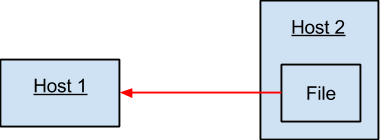
\includegraphics[width=0.4\textwidth]{img/basic_transfer_example.png}
	\caption{Host 1 copying a file.}
\end{figure}
A copy is initiated from Host 1. A file from Host 2 is then transferred to Host 1 using the particular protocol.
\begin{figure}[H]
	\label{fig:interface_example}
	\centering
	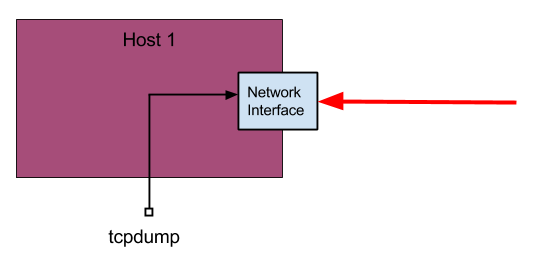
\includegraphics[width=0.5\textwidth]{img/if_example.png}
	\caption{The network interface capturing traffic.}
\end{figure}
The `tcpdump' program (\url{www.tcpdump.org}) comes with most Unix systems. It watches a network interface (e.g eth0) and logs information about packets which pass through. The program is run while the copy is in progress, and the output is filtered to include only packets sent between Host 1 and Host 2.

Note that despite the name, tcpdump can also capture UDP packets, which is relevant for some of the protocols.

\subsubsection{Transfer logging}
The python script for running the file transfers has been written to accept
\begin{itemize}
	\item the name of the network interface
	\item the remote hostname (Host 2)
	\item the path of the file on Host 2
	\item a local path to copy the file to
\end{itemize}

It then resolves the IPs of each host, and for each protocol, runs a copy in isolation. It spawns a tcpdump subprocess, and lets it run for precisely as long as the copy runs. The tcpdump program is started with filters, so that only traffic between the two hosts is captured. It then saves the output in a file.\\\\
\begin{center}
	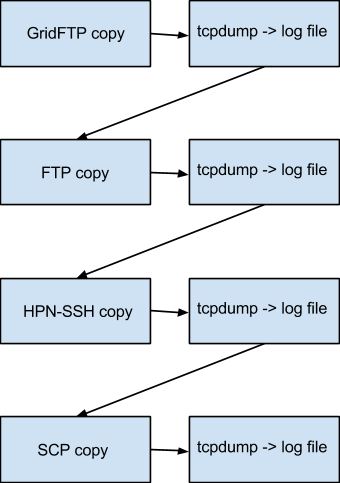
\includegraphics[height=0.5\textheight]{img/seq_example}
\end{center}
Doing it this way allows for a much more controlled environment. Because the tcpdump is only capturing while the copy is running, no other packets will be included in the logs. Also, the copies are run programmatically and consecutively. Following copies are not started until both the tcpdump and protocol processes have been closed, and the log file has been written. This means that they are all run in an identical (within reason) environment, but at the same time do not interfere with each other.\\\\

This test process is run multiple times for statistical reasons, generating multiple log files.

\subsubsection{Analysis of dumps}
A separate python file reads in the log files and parses them. Operations can then be run by looking at the time of each packet, and the size of its payload. This allows analysis of
\begin{itemize}
	\item overhead, because *all* transferred is logged, rather than just the file size
	\item speed (data/time)
	\item consistency
	\item total time
	\item total size
\end{itemize}

This data can then be aggregated over multiple log files, and graphed using the matplotlib python library.\\\\
More info is needed here, and will be filled in once I have completed the analysis scripts.

\bibliographystyle{ACM-Reference-Format-Journals}
\bibliography{ref} 


\end{document}
